Figure \ref{fig:results_varying_samples} shows the accuracy of the different models for various training set sizes, as explained in section \ref{sec:experiments}. Each subset corresponds to a tick in the x axis named \textit{N} which is the number of samples per class for the training split. 

The results of the experiments using MAML and Transfer Learning are grouped according to the dataset with which the pretrained DenseNet model was created.

Prototypical Networks have similar accuracy for LSA16 and CIARP datasets beating the rest of the models for the 5 and 10 samples scenarios, and also the other splits in the case of LSA16. In the case of CIARP, although it did not obtain the best results for all subsets, it achieved a very good performance in all cases, and similar results for the rest of the models.

Regarding RWTH, we can notice that Prototypical Networks cannot take advantage of the images and the accuracy does not increase as the number of samples do. It is possible that Prototypical Networks obtained the lowest accuracy because the images of the hands were unsegmented. In this case, the accuracy of DenseNet is slightly bigger than for other when the number of samples per class, N, is bigger than 15.

On the other hand, we can observe the low accuracy obtained in most experiments that use DenseNet in the subset of 5 samples.

The use of MAML in DenseNet training increses its accuracy in LSA16 and CIARP. However, the use of MAML and Transfer Learning does not bring advantages in the accuracy obtained in RWTH compared to that obtained by the DenseNet model used.

From the obtained results, we can see that the performance of the DenseNet based models increases as more training examples are provided. The use of MAML and Transfer Learning on CIARP and LSA16 means an advantage over the accuracy obtained by the DenseNet model, however it is not so in the case of RWTH. On the other hand, Prototypical Networks models do not show a significant increase in performance as the number of samples increases, always being a good choice with few samples where the hands are segmented.

\begin{figure*}[!ht]
\centering
\begin{tabular}{c}
    \subfigure[Accuracy of Prototypical Networks and DenseNet models trained by varying sample sizes on CIARP taking the results for less than 100 samples.]{
        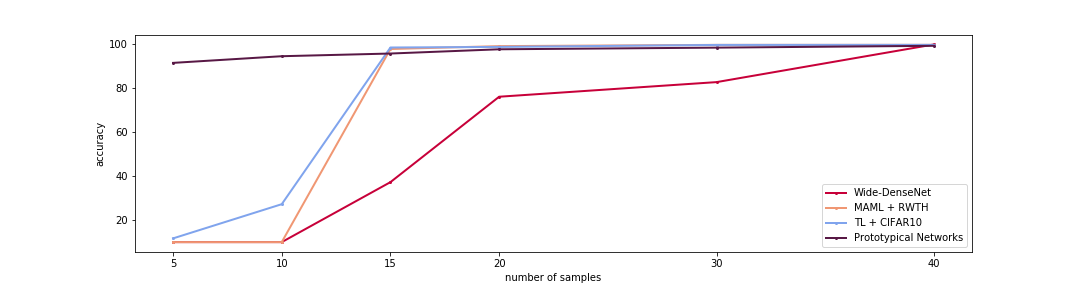
\includegraphics[width=1\textwidth]{results/ciarp.png}
    } \\
    \subfigure[Accuracy of Prototypical Networks and DenseNet models trained by varying sample sizes on LSA16.]{
        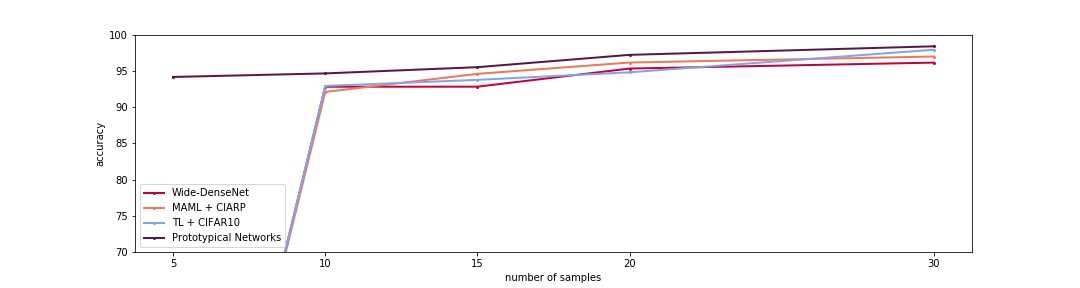
\includegraphics[width=1\textwidth]{results/lsa16.png}
    } \\
    \subfigure[Accuracy of Prototypical Networks and DenseNet models trained by varying sample sizes on LSA16.]{
        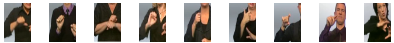
\includegraphics[width=1\textwidth]{results/rwth.png}
    } \\
\end{tabular}
\caption{Accuracy of various models on datasets CIARP, LSA16 and RWTH, respectively. Each plot represents a different dataset, and each line a model that corresponds to the best results obtained on every technique described en section \ref{sec:experiments}. The x-axis indicates the number of samples used to train the model and the y-axis its accuracy. \label{fig:results_varying_samples}}
\end{figure*}
